\chaplbl{Motivation and Demotivation}{sec:motivation}

In order for learners to step out into new and familiar terrain, they
will need encouragement. This section discusses typical ways that
learners are motivated (and can be demotivated!) and describes ways that
communities of practice can be welcoming (or threatening) to new
members.

\seclbl{What Motivates People?}{sec:what-motivates-people}

People learn best when they care about the topic and believe they can
master it. This presents us with a problem because most scientists don't
want to program: they want to do science, and rightly regarding
programming as a tax they have to pay in order to do so. In addition,
their early experiences with programming are often demoralizing, and
believing that something will be hard to learn is a self-fulfilling
prophecy.

Imagine a grid whose axes are labelled ``mean time to master'' and
``usefulness once mastered''. Everything that's quick to master, and
immediately useful should be taught first; things in the opposite corner
that are hard to learn and have little near-term application don't
belong in this course.

\begin{figure}[htbp]
\centering
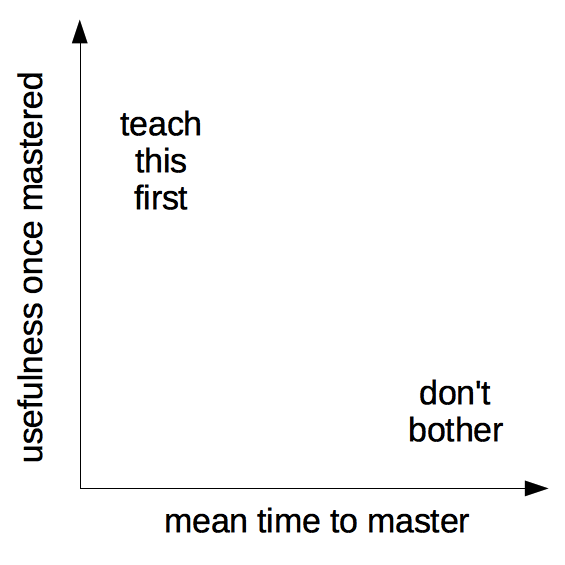
\includegraphics{fig/what-to-teach.png}
\caption{What to Teach}
\end{figure}

\begin{callout}{Actual Time}{callout:actual-time}

Any useful estimate of how long something takes to master must take into
account how frequent failures are and how much time is lost to them. For
example, editing a text file seems like a simple task, but most
graphical editors save things to the user's desktop or home directory.
If people need to run shell commands on the files they've edited, a
substantial fraction won't be able to navigate to the right directory
without help. If this seems like a small problem to you, please revisit
the discussion of expert blind spot \secref{sec:memory}.
\end{callout}

Many of the foundational concepts of computer science, such as
computability, inhabit the ``useful but hard to learn'' corner of the
grid described above. This doesn't mean that they aren't worth learning,
but if our aim is to convince people that they \emph{can} learn this
stuff, and that doing so will help them do more science faster, they are
less compelling than things like automating repetitive tasks.

We have therefore adopted a ``teach most immediately useful first''
approach. We try to have learners do something that \emph{they} think is
useful in their daily work within 15 minutes of starting each lesson.
This not only motivates them, it also helps build their confidence in
us, so that if it takes longer to get to the payoff of a later topic,
they'll stick with us.

Perhaps the best-studied use of this idea is the
media computation approach developed by Guzdial and Ericson at Georgia Tech
\cite{bib:guzdial-mediacomp-retrospective}.
Instead of printing ``hello world'' or summing the first ten integers,
their students' first program opens an image, resizes it to create at
thumbnail, and saves the result. This is an \emph{authentic task}, i.e.,
something that learners believe they would actually do in real life. It
is also \emph{tangible}: if the image comes out the wrong size, learners
have a concrete starting point for debugging.

\begin{challenge}{Authentic Tasks: Think, Pair, Share}{chal:authentic-tasks-think-pair-share}

\textbf{Think} about something you did this week that uses one or more
of the skills we teach, (e.g.~wrote a function, bulk downloaded data,
did some stats in R, forked a repo) and explain how you would use it (or
a simplified version of it) as an exercise or example in class.
\textbf{Pair} up with your neighbor and decide where this exercise fits
on a 2x2 grid of ``short/longtime to master'' and ``low/high
usefulness''? In the class Etherpad, \textbf{share} the task and where
it fits on the 2x2 grid. As a group, we will discuss how these relate
back to our ``teach most immediately useful first'' approach.
\end{challenge}

\seclbl{Strategies for Motivating Learners}{sec:strategies-for-motivating-learners}

\emph{\href{http://www.amazon.com/How-Learning-Works-Research-Based-Jossey-Bass/dp/0470484101/}{How
Learning Works}} contains this list of evidence-based methods to
motivate learners. None of them are surprising---it's hard to imagine
someone saying that we \emph{shouldn't} identify and reward what we
value---but it's useful to check lessons against these points to make
sure they're doing at least a few of these things.

\begin{callout}{Provide an Example}{callout:provide-an-example}

Insert a personal story here about how you establish value in the
classroom. Or, use Rayna's personal story, which goes like this: In the
Unix lesson, we use a haiku to teach grep. This is a great didactic
tool, but it can be hard for learners to see how they can use it in
their research. After the grep lesson, I show a one liner that combines
\texttt{head}, \texttt{grep}, \texttt{sort}, and \texttt{uniq} to
produce a ranked list of the most abundant sequences. I emphasize that
the students just learned each of the pieces (see
\href{https://wikis.utexas.edu/display/bioiteam/Scott's list of linux one-liners}).
This way, I connect my bioinformatics users with domain-specific
examples using an authentic task that is relevant to their research.
\end{callout}

\begin{challenge}{Brainstorming Motivational Strategies}{chal:brainstorming-motivational-strategies}

\emph{Think} back to a computational (or other) course you took in the
past, and identify one thing the instructor did that motivated you.
\emph{Pair} up with your neighbor and discuss what motivated you.
\emph{Share} the motivational story in the Etherpad.
\end{challenge}

\begin{callout}{Not Just Learners}{callout:not-just-learners}

What's missing from this list is strategies to motivate the
\emph{instructor}. As we said in \secref{sec:intro},
learners respond to an instructor's enthusiasm, and instructors need to
care about a topic in order to keep teaching it, particularly when they
are volunteers.
\end{callout}

\begin{challenge}{Why Do You Teach?}{chal:why-do-you-teach}

We all have a different motivation for teaching, and that is a really
good thing! SWC wants instructors with diverse backgrounds because you
each bring something unique to our community. After this
class, or during a break, write a short explanation of what motivates
you to teach. Save this as part of your teaching philosophy for future
reference.
\end{challenge}

\seclbl{Demotivation}{sec:demotivation}

As noted in \secref{sec:intro}, we are privileged: most of our learners are physically
safe, well fed, well educated, and highly motivated. Our challenge is
therefore not demotivating them.

A few common demotivators are \emph{indifference} and \emph{unfairness}.
If learners believe that the instructor or the educational system
doesn't care about them or the lesson, they won't care either. And if
people believe the class is unfair, they will also be demotivated, even
if it is unfair in their favor (because consciously or unconsciously
they will worry that they will some day find themselves in the group on
the losing end). Finally, a ``holier-than-thou'' or contemptuous
attitude from an instructor is a quick way to alienate a classroom and
cause learners to tune out.

\begin{callout}{Things You Shouldn't Do in a Workshop}{callout:things-you-shouldnt-do-in-a-workshop}

\begin{itemize}
\item
  Tell learners they are rubbish because they use Excel and/or Word,
  don't modularize their code, etc.
\item
  Repeatedly make digs about Windows and praise Linux, e.g., say that
  the former is for amateurs.
\item
  Criticize GUI applications (and by implication their users) and
  describe command-line tools as the One True Way.
\item
  Dive into complex or detailed technical discussion with the one or two
  people in the audience who clearly don't actually need to be there.
\item
  Pretend to know more than you do. People will actually trust you more
  if you are frank about the limitations of your knowledge, and will be
  more likely to ask questions and seek help.
\item
  Use the J word (``just''). As discussed in \secref{sec:memory}, this
  signals to the learner that the instructor thinks their problem is
  trivial and by extension that they therefore must be stupid for not
  being able to figure it out.
\item
  Feign surprise. Saying things like ``I can't believe you don't know
  X'' or ``you've never heard of Y?'' signals to the learner that they
  do not have some required pre-knowledge of the material you are
  teaching, that they are in the wrong place, and it may prevent them
  from asking questions in the future. (This idea is due to the Recurse
  Center's \href{https://www.recurse.com/manual\#sec-environment}{Social
  Rules}).
\end{itemize}
\end{callout}

\begin{callout}{The Importance of Having Rules}{callout:the-importance-of-having-rules}

Software Carpentry and Data Carpentry share a
Code of Conduct, and all
participants in our workshops are required to abide by it. Its details
are important, but the most important thing about it is that it exists:
knowing that we have rules tells people a great deal about our values
and about what kind of learning experience they can expect.
\end{callout}

\begin{callout}{Stereotype Threat}{callout:stereotype-threat}

Reminding people of negative stereotypes, even in subtle ways, makes
them anxious about the risk of confirming those stereotypes, which in
turn reduces their performance. This is called
\emph{\href{https://en.wikipedia.org/wiki/Stereotype\_threat}{stereotype
threat}}, and the clearest examples in computing are gender-related.
Depending on whose numbers you trust, only 12-18\% of programmers are
women, and those figures have actually been getting worse over the last
20 years. There are many reasons for this (see Margolis and Fisher's
\emph{\href{http://www.amazon.com/Unlocking-Clubhouse-Computing-Jane-Margolis/dp/0262632691/}{Unlocking
the Clubhouse}} and Margolis's
\emph{\href{https://www.amazon.com/Stuck-Shallow-End-Education-Computing/dp/0262514044/}{Stuck
in the Shallow End}}), and Steele's
\emph{\href{http://www.amazon.com/dp/0393339726/}{Whistling Vivaldi}}
summarizes what we know about stereotype threat in general and presents
some strategies for mitigating it in the classroom.

However, while there's lots of evidence that unwelcoming climates
demotivate members of under-represented groups, it's not clear that
stereotype threat is the underlying mechanism. Part of the problem is
that
\href{http://www.europhd.net/html/\_onda02/07/PDF/20th\_lab\_materials/jane/shapiro\_neuberg\_2007.pdf}{the
term has been used in many ways}; another is
\href{https://www.psychologytoday.com/blog/rabble-rouser/201512/is-stereotype-threat-overcooked-overstated-and-oversold}{questions
about the replicability of key studies}. What \emph{is} clear is that we
need to aovid thinking in terms of a deficit model (i.e., we need to
change the members of under-represented groups because they have some
deficit, such as lack of prior experience) and instead use a systems
approach (i.e., we need to change the system because it produces these
disparities).
\end{callout}

\begin{challenge}{Brainstorming Demotivational Experiences}{chal:brainstorming-demotivational-experiences}

\emph{Think} back to a time when you demotivated a student (or when you
were demotivated as a student). \emph{Pair} up with your neighbor and
discuss what you could have done differently in the situation.
\emph{Share} the demotivational story in the Etherpad.
\end{challenge}

\begin{callout}{Never Learn Alone}{callout:never-learn-alone}

One way to support at-risk learners of all kinds is to have people sign
up for workshops in small teams rather than as individuals. If an entire
lab group comes, or if attendees are drawn from the same (or
closely-related) disciplines, everyone in the room will know in advance
that they will be with at least a few people they trust, which increases
the chances of them actually coming. It also helps after the workshop:
if people come with their labmates, they can work together to implement
what they've learned.
\end{callout}

\seclbl{Impostor Syndrome}{sec:impostor-syndrome}

\href{https://en.wikipedia.org/wiki/Impostor\_syndrome}{Impostor
syndrome} is the belief that one is not good enough for a job or
position, that one's achievements are lucky flukes, and an accompanying
fear of being ``found out''. Impostor syndrome seems to be particularly
common among
\href{https://www.usenix.org/blog/impostor-syndrome-proof-yourself-and-your-community}{high
achievers who undertake publicly visible work}.

Academic work is frequently undertaken alone or in small groups but the
results are shared and criticized publicly. In addition, we rarely see
the struggles of others, only their finished work, which can feed the
belief that everyone else finds it easy. Women and minority groups, who
already feel additional pressure to prove themselves in some settings,
\href{http://www.paulineroseclance.com/pdf/ip\_high\_achieving\_women.pdf}{may
be particularly affected}.

Two ways of dealing with your own impostor syndrome are:

\begin{enumerate}
\item
  Ask for feedback from someone you respect and trust. Ask them for
  their honest thoughts on your strengths and achievements, and commit
  to believing them.
\item
  Look for role models. Who do you know who presents as confident and
  capable? Think about how they conduct themselves. What lessons can you
  learn from them? What habits can you borrow? (Remember, they quite
  possibly also feel as if they are making it up as they go.)
\end{enumerate}

As an instructor, you can help people with their impostor syndrome by
sharing stories of mistakes that you have made or things you struggled
to learn. This reassures the class that it's OK to find topics hard.
Being open with the group makes it easier to build trust and make
students confident to ask questions. (Live coding is great for this:
typos let the class see you're not superhuman.)

You can also emphasize that you want questions: you are not succeeding
as a teacher if no one can follow your class, so you're asking students
for their help to help you learn and improve. Remember, it's much more
important to \emph{be} smart than to \emph{look} smart.

The Ada Initiative has
\href{http://adainitiative.org/continue-our-work/impostor-syndrome-training/}{some
excellent resources} for teaching about and dealing with imposter
syndrome.

\seclbl{Mindset}{sec:mindset}

Learners can be demotivated in subtler ways as well. For example, Dweck
and others have studied the differences of
\href{https://en.wikipedia.org/wiki/Mindset\#Fixed\_mindset\_and\_growth\_mindset}{fixed
mindset and growth mindset}. If people believe that competence in some
area is intrinsic (i.e., that you either ``have the gene'' for it or you
don't), \emph{everyone} does worse, including the supposedly advantaged.
The reason is that if they don't get it at first, they figure they just
don't have that aptitude, which biases future performance. On the other
hand, if people believe that a skill is learned and can be improved,
they do better on average.

A person's mindset can be shaped by subtle cues. For example, if a child
is told, ``You did a good job, you must be very smart,'' she is likely
to develop a fixed mindset. If on the other hand she is told, ``You did
a good job, you must have worked very hard,'' she is likely to develop a
growth mindset, and subsequently achieve more. Studies have also shown
that the simple action of telling learners about the different mindsets
before a course can improve learning outcomes for the whole group.

\seclbl{Accessibility}{sec:accessibility}

Not providing equal access to lessons and exercises is about as
demotivating as it gets. If you look at
\href{http://swcarpentry.github.io/v4/python/flow.html}{our old lesson
on Python}, for example, you'll find that the text beside the slides
includes all of the narration---but none of the Python source code.
Someone using a
\href{https://en.wikipedia.org/wiki/Screen\_reader}{screen reader} would
therefore be able to hear what was being said about the program, but
wouldn't know what the program actually was.

While it may not be possible to accommodate everyone's needs, it
\emph{is} possible to get a good working structure in place without any
specific knowledge of what specific disabilities people might have.
Having at least some accommodations prepared in advance also makes it
clear that hosts and instructors care enough to have thought about
problems in advance, and that any additional concerns are likely to be
addressed.

\begin{callout}{It Helps Everyone}{callout:it-helps-everyone}

\href{https://en.wikipedia.org/wiki/Curb\_cut}{Curb cuts} (the small
sloped ramps joining a sidewalk to the street) were originally created
to make it easier for the physically disabled to move around, but proved
to be equally helpful to people with strollers and grocery carts.
Similarly, steps taken to make lessons more accessible to people with
various disabilities also help everyone else. Proper captioning of
images, for example, doesn't just give screen readers something to say:
it also makes the images more findable by exposing their content to
search engines.
\end{callout}

The first step is to know what you need to do. The
\href{http://www.w3.org/WAI/training/accessible}{W3C Accessibility
Initiative's checklist for presentations} is a good starting point
focused primarily on assisting the visually impaired, while Liz Henry's
blog post about
\href{https://modelviewculture.com/pieces/unlocking-the-invisible-elevator-accessibility-at-tech-conferences}{accessibility
at conferences} has a good checklist for people with mobility issues,
and
\href{https://modelviewculture.com/pieces/qa-making-tech-events-accessible-to-the-deaf-community}{this
interview} with Chad Taylor is a good introduction to issues faced by
the hearing impaired.

The second is to know how well you're doing. For example, sites like
\href{http://webaim.org/}{WebAIM} allow you to check how accessible your
online materials are to visually impaired users. (According to
\href{http://wave.webaim.org/report\#/software-carpentry.org}{this
report}, we still have some work to do\ldots{})

The third, and most important, is to \emph{involve people with
disabilities in decision-making}. Our mailing lists are a good place to
ask for advice, and updates to
\href{http://software-carpentry.org/workshops/checklists/accessibility/}{our
accessibility checklist} are always welcome.

\begin{callout}{Every Little Bit Counts}{callout:every-little-bit-counts}

Looking at people who work with disability and accessibility, it's easy
to be overwhelmed by all the different ways we could make instruction
more accessible. \emph{Don't panic.} Instead:

\begin{itemize}
\item
  \emph{Don't do everything at once.} We don't ask learners in our
  workshops to adopt all our best practices or tools in one go, but
  instead to work things in gradually at whatever rate they can manage.
  Similarly, try to build in accessibility habits when preparing for
  workshops by adding something new each time.
\item
  \emph{Do the easy things first.} There are plenty of ways to make
  workshops more accessible that are both easy and don't create extra
  cognitive load for anyone: font choices, general text size, checking
  in advance that your room is accessible via an elevator or ramp, etc.
\end{itemize}
\end{callout}

\begin{callout}{Accessibility Testing}{callout:accessibility-testing}

Find the nearest public transportation drop-off point to your building
and walk from there to your office and then to the nearest washroom,
making notes about things you think would be difficult for someone with
mobility issues. Now borrow a wheelchair and repeat the journey. How
complete was your list of challenges? And did you notice that the first
sentence in this challenge assumed you could actually walk?
\end{callout}

\seclbl{Inclusivity}{sec:inclusivity}

\emph{Inclusivity} is a policy of including people who might otherwise
be excluded or marginalized. In computing, it means making a positive
effort to be more welcoming to women, people of color, people with
various sexual orientations, the elderly, the physically challenged, the
formerly incarcerated, the economically disadvantaged, and everyone else
who doesn't fit Silicon Valley's white/Asian male demographic. Lee's
paper
``What can I do today to create a more inclusive community in CS?''
\cite{bib:lee-create-inclusive-community}
is a brief, practical guide to
doing that with references to the research literature. These help
learners who belong to one or more margainalized or excluded groups, but
help motivate everyone else as well; while they are phrased in terms of
term-long courses, many can be applied in our workshops, such as:

\begin{itemize}
\item
  asking learners to email you before the workshop to explain how they
  believe the training could help them achieve their goals;
\item
  reviewing notes to make sure they are free from gendered pronouns,
  that they include culturally diverse names, etc.;
\item
  emphasize that what matters is the rate at which they are learning,
  not the advantages or disadvantages they had when they started;
\item
  encouraging pair programming; and
\item
  actively mitigate behavior that some learners may find intimidating,
  e.g., use of jargon or ``questions'' that are actually asked to
  display knowledge.
\end{itemize}

\begin{challenge}{Pick One}{chal:pick-one}

\begin{enumerate}
\item
  Pick one activity or change in practice from
  Lee's paper \cite{bib:lee-create-inclusive-community}
  that you would like to work on.
\item
  Put a reminder in your calendar three months in the future to
  self-check whether you have done something about it.
\end{enumerate}
\end{challenge}
